\providecommand{\main}{../../../..}
\documentclass[\main/dresen_thesis.tex]{subfiles}
\begin{document}
  \label{sec:doublelayers:magnetism:intro}
  The magnetic field that is produced by a homogeneously magnetized layer of nanocubes in a square array at a position in vertical distance $z \eq \tilde{z} a$, given in units of the square array lattice constant $a$, can be estimated by evaluating the sum of dipole fields produced by each of the respective nanocubes in a infinitely extending lattice via
  \begin{align}
    \begin{split}
      \vec{B} \eq& \sum_{i,\, j \eq -\infty}^\infty \frac{\mu_0}{4 \pi} \frac{3 \vec{r}_{ij} (\vec{\mu}_{ij} \cdot \vec{r}_{ij}) - r_{ij}^2 \vec{\mu}_{ij}}{r_{ij}^5},\\
      \vec{r}_{ij} \eq& a \begin{pmatrix}-i\\-j\\\tilde{z}\end{pmatrix}, \hspace{1cm}
      \vec{\mu}_{ij} \eq \mu \begin{pmatrix}1\\0\\0\end{pmatrix}.
    \end{split}
  \end{align}

  Due to symmetry, the $B_y$ and $B_z$ component vanish and only the $B_x$ component remains, which is determined by the sum
  \begin{align}
    B_x \eq& \frac{\mu_0 \mu}{4 \pi a^3} \sum_{i,\, j \eq -\infty}^\infty  \frac{2 i^2 - j^2 - \tilde{z}^2}{(i^2 + j^2 + \tilde{z}^2)^{5/2}}.\\
  \end{align}
  Using the symmetry of the square lattice further, the summation can be reduced to
  \begin{align}
    B_x \eq& \frac{\mu_0 \mu}{4 \pi a^3} \biggl( -\frac{1}{\tilde{z}^3} + 2 \sum_{i \eq 1}^\infty \frac{i^2 - 2\tilde{z}^2}{(i^2 + \tilde{z}^2)^{5/2}} + 4 \sum_{i,\, j \eq 1}^\infty  \frac{2 i^2 - j^2 - \tilde{z}^2}{(i^2 + j^2 + \tilde{z}^2)^{5/2}} \biggr).\\
  \end{align}

  The prefactor of the sum determines the order of magnitude for the field strength and for nanocubes such as Ac-CoFe-C with a magnetic moment in the order of $\mu \eq 23000 \mu_B$ and a lattice constant of $a \eq 13 \unit{nm}$, it is given by $9.7 \unit{mT}$.
  Solving the sum numerically, the magnetic field of a nanocube layer with respect to $\tilde{z}$ is obtained as shown in \reffig{fig:doubleLayers:layerMagneticField}.
  The infinite sum was aborted at a lattice extension of $1000$ sites as convergence was good enough at this point and increasing the lattice by ten-fold changed the result by only $1\%$.

  \begin{figure}[tb]
    \centering
    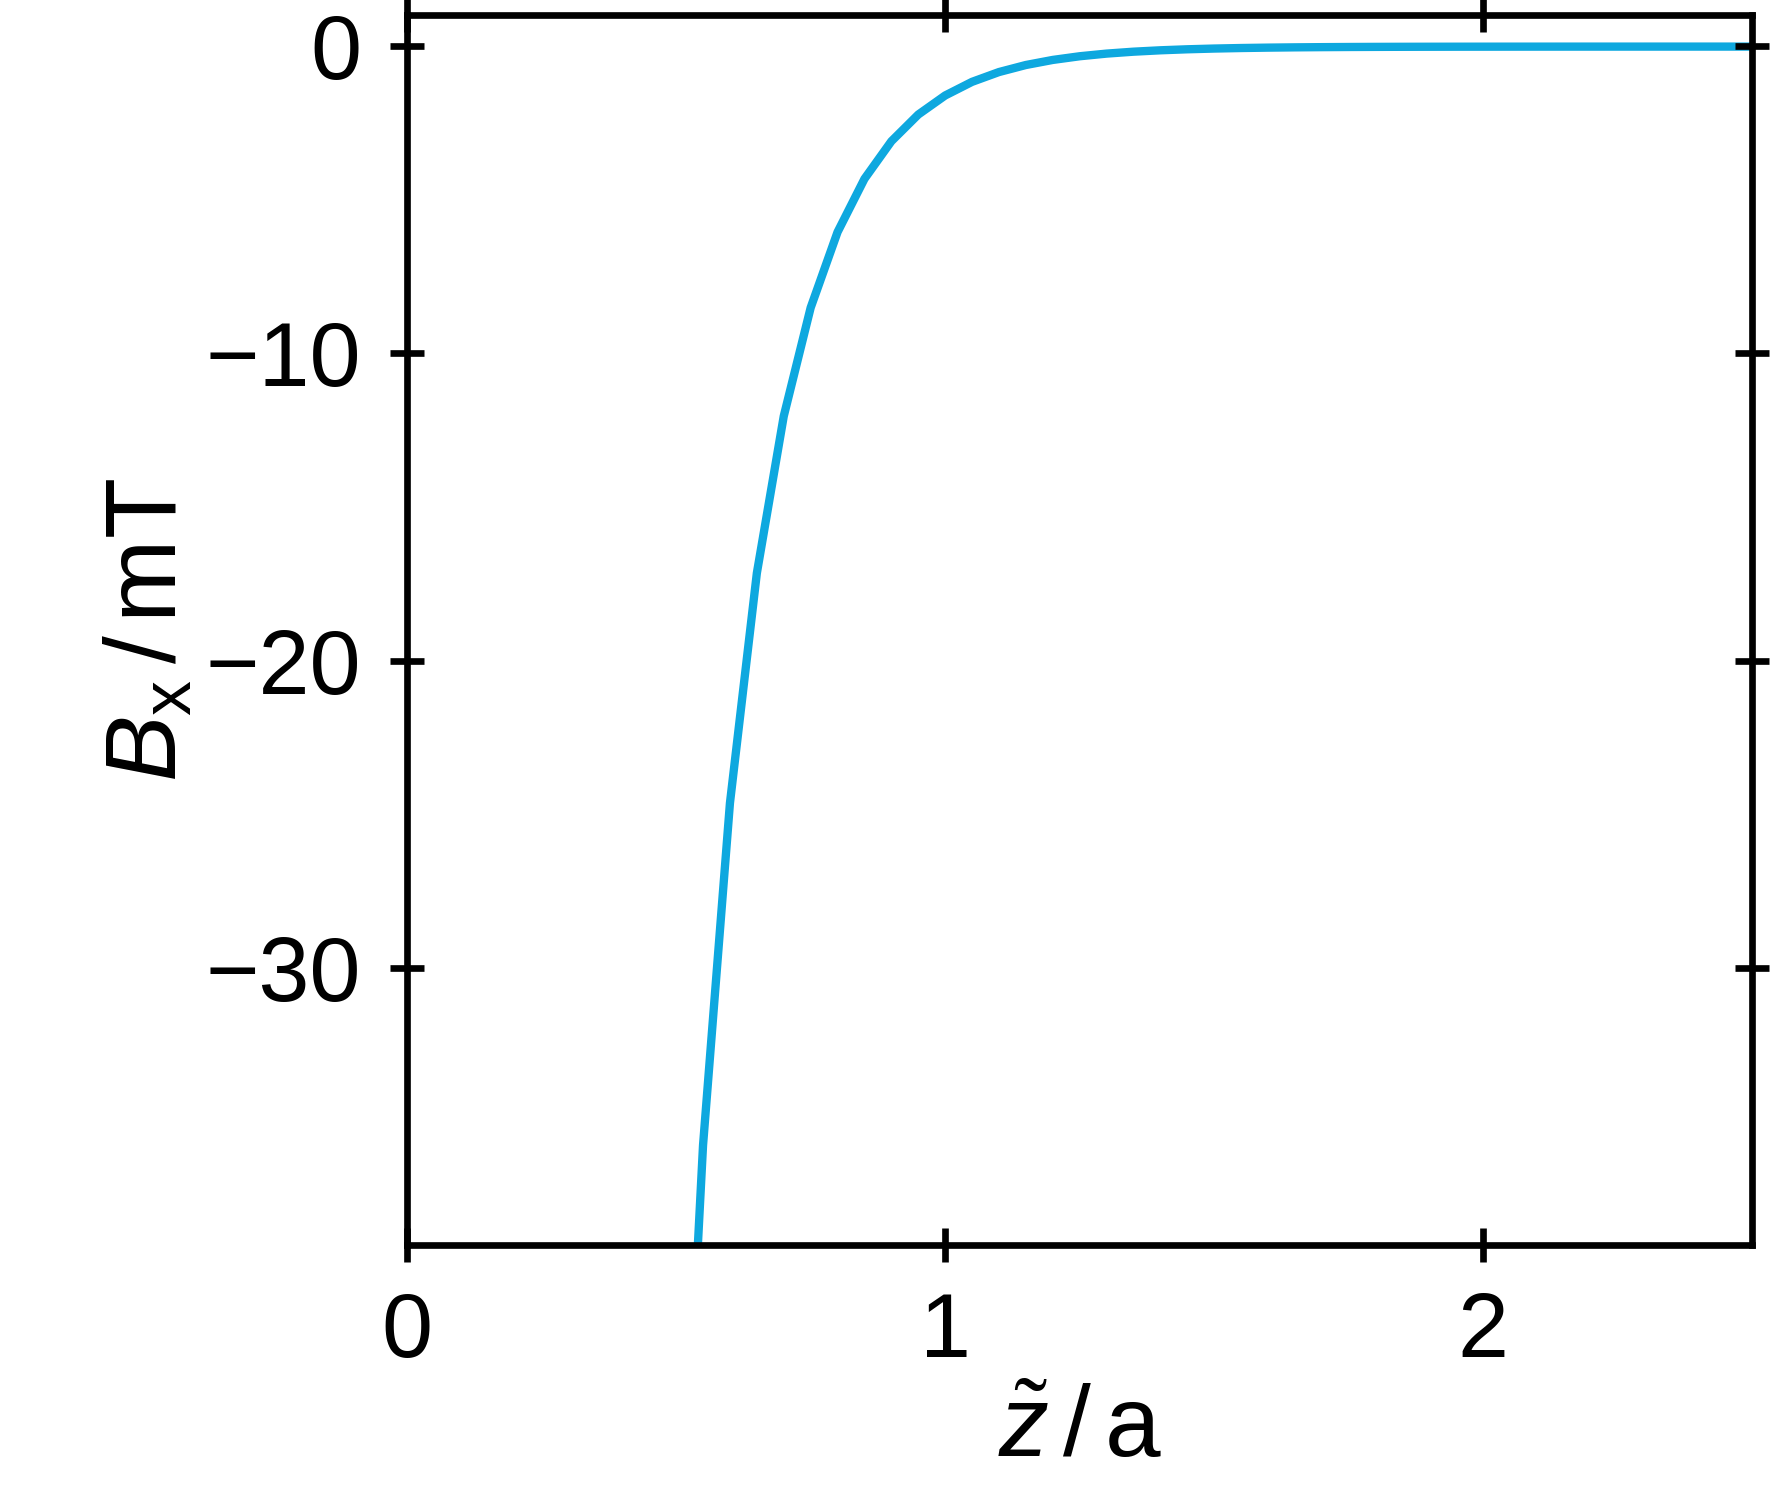
\includegraphics{doublelayers_simulatedFieldStrenghs}
    \caption{\label{fig:doubleLayers:layerMagneticField}Magnetic field $B_x$ produced by a layer of nanocubes, with each magnetized along $x$, and in a square lattice with lattice constant $a$. The field is given with respect to the vertical distance $\tilde{z}$ in units of the lattice constant.}
  \end{figure}                                                    

  From the calculation it is visible that the produced magnetic field of an fully magnetized square array rapidly falls off in magnitude already at a distance of one lattice length.
  Therefore dipolar interlayer effects should be expected in the discussed samples only at close proximity of the nanolayers.
  Then the produced field generates a field that points into the antiparallel direction as the magnetization of producing layer and can therefore be considered like an antiferromagnetic coupling.
\end{document}